\documentclass[11pt]{article}
\usepackage{amsmath, amssymb, amscd, amsthm, amsfonts}
\usepackage{graphicx}
\usepackage{hyperref}
\hypersetup{
    colorlinks=true,
    linkcolor=blue,
    filecolor=magenta,      
    urlcolor=cyan,
    pdftitle={Overleaf Example},
    pdfpagemode=FullScreen,
    }
\usepackage[dvipsnames]{xcolor}

\oddsidemargin 0pt
\evensidemargin 0pt
\marginparwidth 40pt
\marginparsep 10pt
\topmargin -20pt
\headsep 10pt
\textheight 8.7in
\textwidth 6.65in
\linespread{1.2}

\title{Course Report: Time Series and Survival Analysis}
\author{Nan He}
\date{}

\newtheorem{theorem}{Theorem}
\newtheorem{lemma}[theorem]{Lemma}
\newtheorem{conjecture}[theorem]{Conjecture}

\newcommand{\rr}{\mathbb{R}}

\newcommand{\al}{\alpha}
\DeclareMathOperator{\conv}{conv}
\DeclareMathOperator{\aff}{aff}

\begin{document}

\maketitle

%\begin{abstract}
%(Abs)
%\end{abstract}

\section{Main objective of the analysis}\label{section-introduction-1}
Acknowledgement: this is a course project for \href{https://www.coursera.org/professional-certificates/ibm-machine-learning}{IBM Machine Learning professional certificate}. The project notebook can be accessed \href{https://github.com/henankf223/Assignment-6-TS/blob/40f8f0d003b55ed7d9246c2828d0f25b7517e229/Assignmeng_6_TS_stock.ipynb}{here}.

In this report, the data I will be using is the stock price time series data for Apple (AAPL), Boeing (BA), and Walmart (WMT) during 2017-1 and 2018-1, the data are acquired  \href{https://www.kaggle.com/szrlee/stock-time-series-20050101-to-20171231s}{here}.
\textbf{The goal of this report is to use time series methods to forecast the stock price in one month.}

The target includes: 

\begin{itemize}
\item Prepare an clean the data for modeling.
\item Train different time series models on those three stock price series.
\item Forecast one month into the future, comparing the predictions with the actual stock price.
\end{itemize}

I will be using both \textbf{smoothing methods}, \textbf{ARIMA}, and \textbf{SARIMA} for modeling.
There are \textbf{some possible snags} that can be problematic for the analysis including:

\begin{itemize}
\item Stock price has strong trend and vague seasonality, the assumption is difficult to make.
\item It is doubt that whether stock price solely depends on past data? I would consider not.
\end{itemize}

Those problems can be addressed by:

\begin{itemize}
\item I will assume an close-to-linear up-going trend, and a monthly seasonality (since weekly seasonality is to short for predictions).
\item Due to the nature of the stock market, the prediction cannot be very accurate. We should focus mainly on some general patterns and trends.
\end{itemize}

\section{Description of the data set}\label{section-introduction-2}
The original data set is the stock price for 30 different companies from 2017 to 2018. I took Apple (AAPL), Boeing (BA), and Walmart (WMT), representing different sectors.
The following is a \textbf{data dictionary}. 
The feature columns are:

\begin{itemize}
\item Date: the date label
\item Open: the open price
\item High: the highest price of the day
\item Low: the lowest price of the day
\item Close: the close price
\item Volume: the trade volume
\item Name: the name/label of the stock
\end{itemize}
%\newpage

The date is a date label that can be converted to date-time, the Open, High, Low, Close are in float64, and Volume is int. The Name is a string object.

\section{Data exploration, cleaning, and feature engineering}\label{section-introduction-3}
The data need to be cleaned. Here is the list of actions I took:

\begin{itemize}
\item Separate each Name into a single dataframe. making three dataframe characterizing AAPL, BA, and WMT. 
\item Drop "Name", "Volume". Since they are not related with our goal.
\item Convert data to pandas datetime.
\item Check NaN, fill with average data from the previous and next day.
\end{itemize}

The example data after cleaning looks like:

\begin{figure}[h!]
\centerline{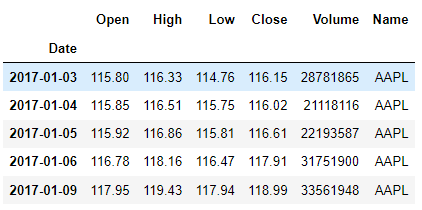
\includegraphics[scale=0.7]{ts_1.png}}
\caption{AAPL stock price data example.}
\end{figure}

The data after cleaning contains 251 data labels for each stock.
Here are plots for all three stock, taking the Close price of each day:

\begin{figure}[h!]
\centerline{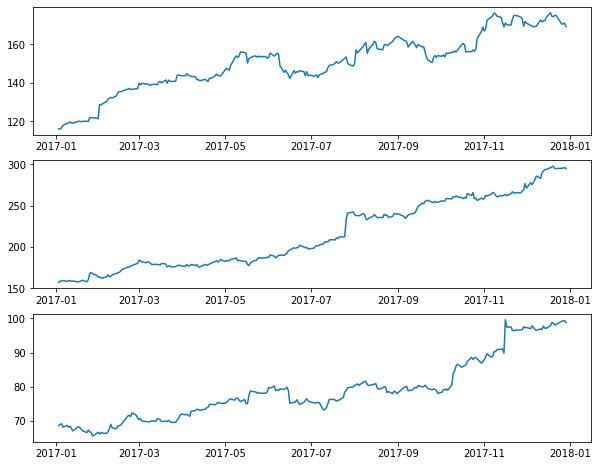
\includegraphics[scale=0.7]{ts_2.png}}
\caption{Close price for AAPL, BA, and WMT from 2017-1 to 2018-1.}
\end{figure}

There are some interesting observations here, for example:
\begin{itemize}
\item There is a clear growing trend in this series. It is necessary to assume a linear trend or conduct differencing.
\item The data have some sudden changes, for example, WMT has a steep growth in 2017-11. It needs to be very carefully considered when choosing seasonality.
\end{itemize}

\section{Stationary, and the assumptions about trend and seasonality.}\label{section-dsmoothing}
In this report, I take the "Close" price of everyday for time-series modelling.
Before going into modeling, I firstly confirmed that the stock series is non-stationary.
To take account for the trend and seasonality, I have to make the following assumptions:

\begin{itemize}
\item Their trends are additive, each components are linear.
\item The seasonal components are additive, the period is either 5 days or 21 days. This is a rough estimation, and we will test whether the seasonal components is necessary.
\end{itemize}

The data is then split into train and test set, including 230 and 21 labels, respectively.
Every model below will be trained on the train set, and forecast one month (21 days) into the further.
The prediction results will be compared with the test set; their mean square error (MSE) will be used as the evaluation metric.
In the next four sections, four different type of models will be trained, and forecast on the test set.

\newpage

\section{Double Exponential Smoothing}\label{section-dsmoothing}

\begin{figure}[h!]
\centerline{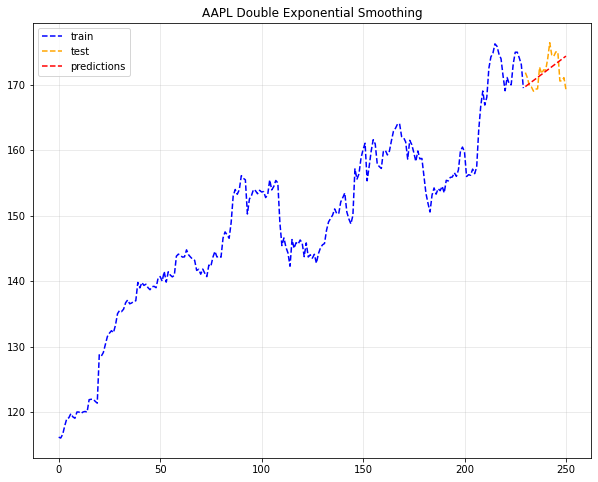
\includegraphics[scale=0.5]{des_1.png}}
\caption{Double exponential smoothing for AAPL training on 2017-1 to 2017-12, predicting 2018-1.}
\end{figure}

\begin{figure}[h!]
\centerline{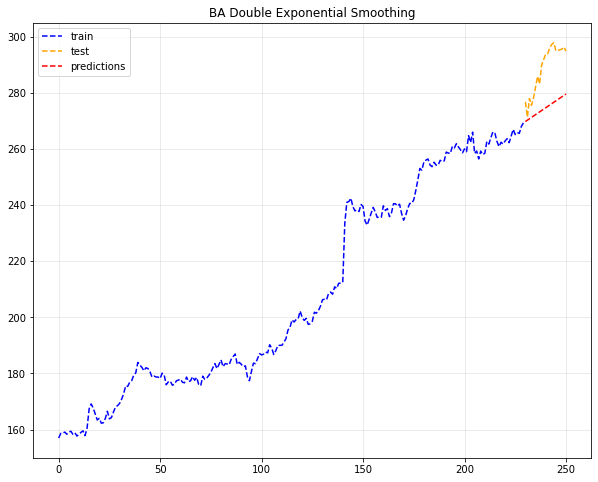
\includegraphics[scale=0.5]{des_2.png}}
\caption{Double exponential smoothing for BA training on 2017-1 to 2017-12, predicting 2018-1.}
\end{figure}

\begin{figure}[h!]
\centerline{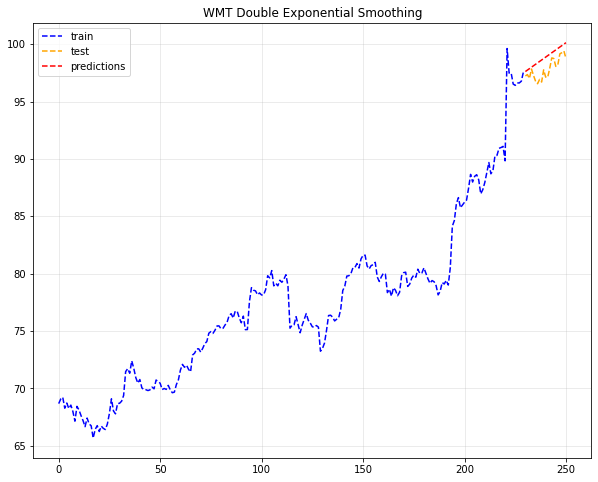
\includegraphics[scale=0.5]{des_3.png}}
\caption{Double exponential smoothing for WMT training on 2017-1 to 2017-12, predicting 2018-1.}
\end{figure}

\newpage

\section{Triple Exponential Smoothing}\label{section-tsmoothing}

\begin{figure}[h!]
\centerline{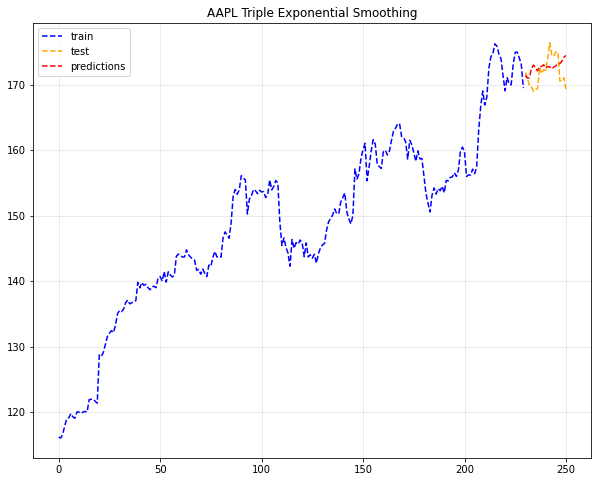
\includegraphics[scale=0.5]{tes_1.png}}
\caption{Triple exponential smoothing for AAPL training on 2017-1 to 2017-12, predicting 2018-1.}
\end{figure}

\begin{figure}[h!]
\centerline{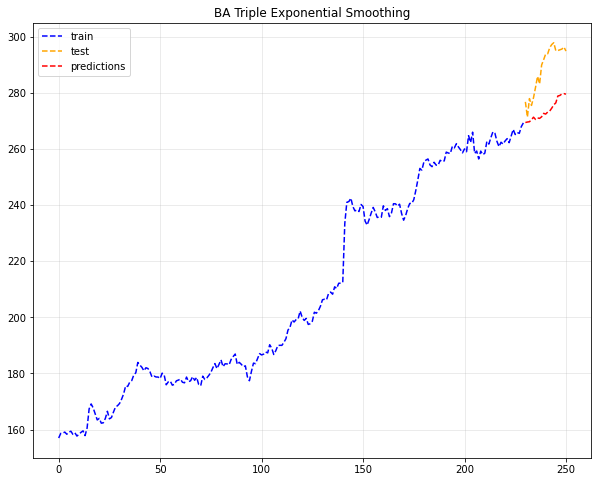
\includegraphics[scale=0.5]{tes_2.png}}
\caption{Triple exponential smoothing for BA training on 2017-1 to 2017-12, predicting 2018-1.}
\end{figure}

\begin{figure}[h!]
\centerline{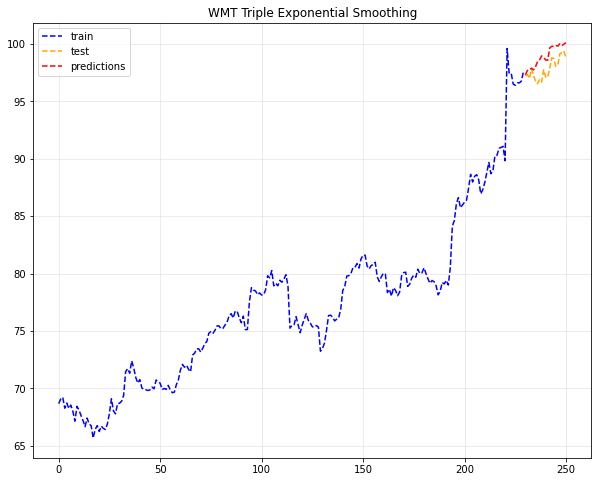
\includegraphics[scale=0.5]{tes_3.png}}
\caption{Triple exponential smoothing for WMT training on 2017-1 to 2017-12, predicting 2018-1.}
\end{figure}

\newpage

\section{ARIMA}\label{section-arima}
The ARIMA model needs to determine the AR, I, and MA orders. I do it by ploting the Autocorrelation and Partial-Autocorrelation Functions (ACF and PACF).
Here I take one example to show the parameter tuning process:
Start with AAPL, the ACF and PACF plots are:

\begin{figure}[h!]
\centerline{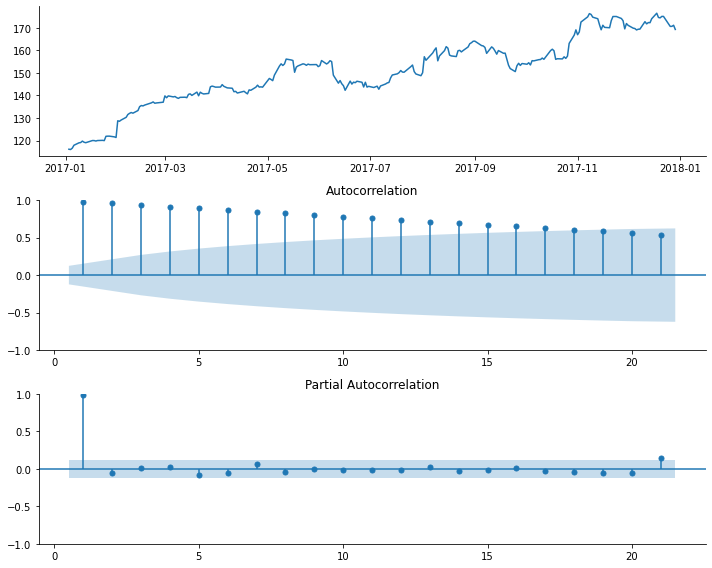
\includegraphics[scale=0.5]{arima1.png}}
\caption{AAPL ACF and PACF plots.}
\end{figure}

\begin{itemize}
\item The autocorrelation is large, try using difference I=1.
\item Following the Box-Jenkins procedure, I choose a AR + MA model, with order=1, determined from the PACF plots.
\end{itemize}

\newpage

Here is the statistical summary of a (1,1,1) model:

\begin{figure}[h!]
\centerline{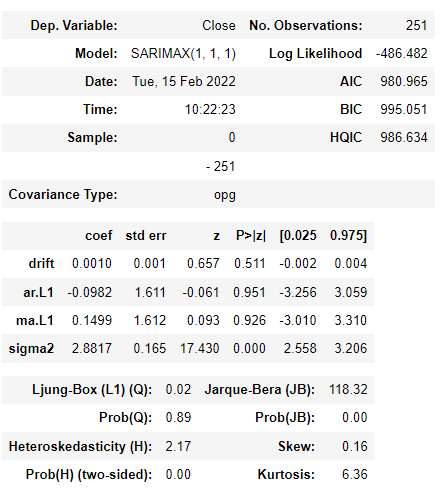
\includegraphics[scale=0.45]{arima2.png}}
\caption{AAPL AR=1, I=1, MA=1 model statistics.}
\end{figure}

The residue also looks ok:

\begin{figure}[h!]
\centerline{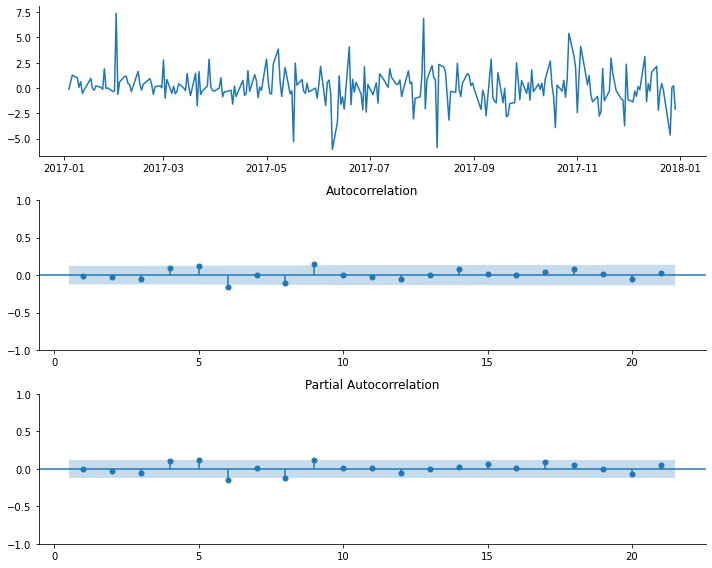
\includegraphics[scale=0.45]{arima3.png}}
\caption{AAPL AR=1, I=1, MA=1 model residue, ACF, and PACF.}
\end{figure}

So the model I will be using for AAPL is (1,1,1), similar procedures are conducted BA and WMT, too.
I tested their forecast the same way as previous smoothing models:

\begin{figure}[h!]
\centerline{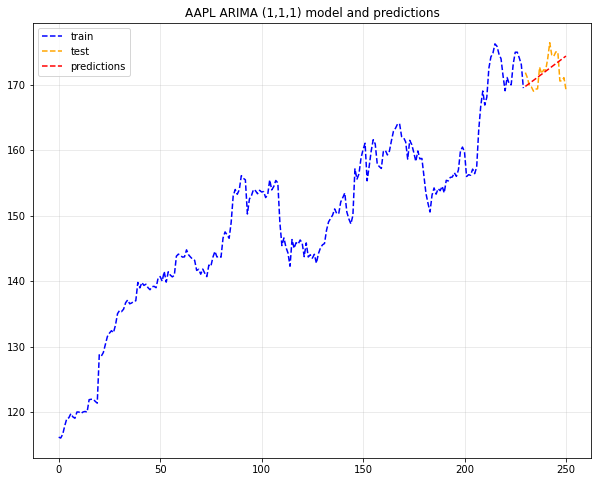
\includegraphics[scale=0.5]{arima_p1.png}}
\caption{AAPL ARIMA (1,1,1) model, training on 2017-1 to 2017-12, predicting 2018-1.}
\end{figure}

\begin{figure}[h!]
\centerline{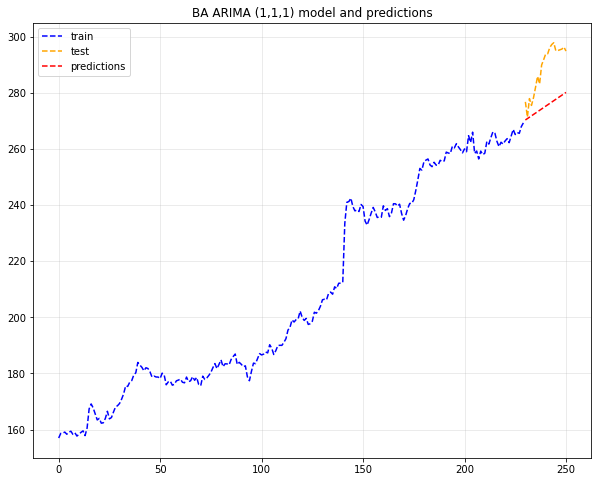
\includegraphics[scale=0.5]{arima_p2.png}}
\caption{BA ARIMA (1,1,1) model, training on 2017-1 to 2017-12, predicting 2018-1.}
\end{figure}

\begin{figure}[h!]
\centerline{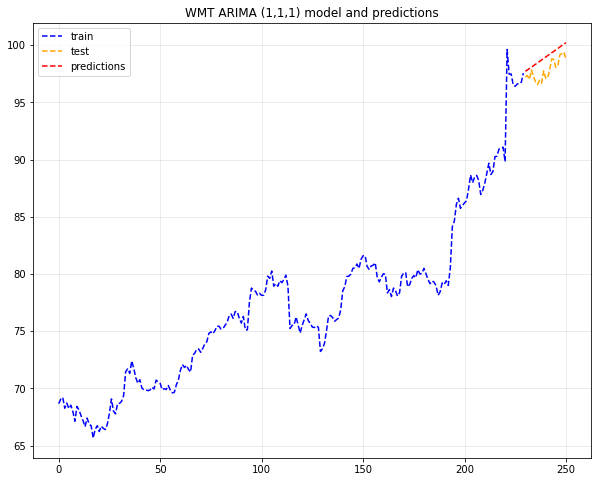
\includegraphics[scale=0.5]{arima_p3.png}}
\caption{WMT ARIMA (1,1,1) model, training on 2017-1 to 2017-12, predicting 2018-1.}
\end{figure}

\newpage

\section{SARIMA}\label{section-sarima}

The SARIMA model adds seasonal components to ARIMA. As we assumed before, a 21-day seasonality will be considered. The parameter is also (1,1,1).

\begin{figure}[h!]
\centerline{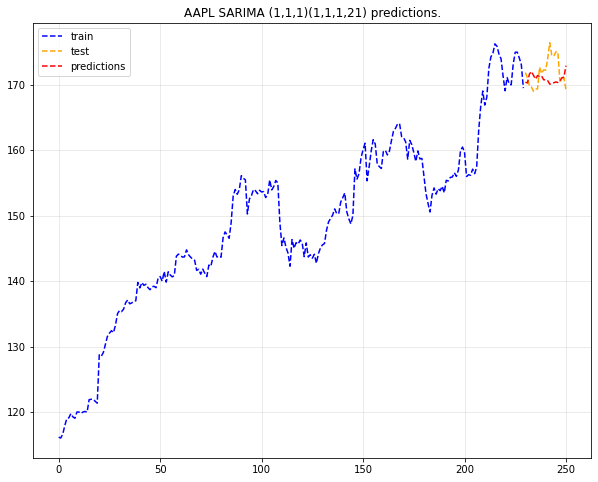
\includegraphics[scale=0.5]{sarima_p1.png}}
\caption{AAPL SARIMA (1,1,1)(1,1,1,21) model, training on 2017-1 to 2017-12, predicting 2018-1.}
\end{figure}
\begin{figure}[h!]
\centerline{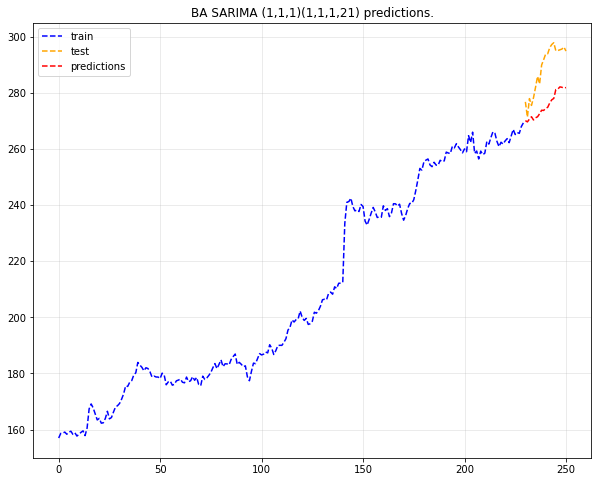
\includegraphics[scale=0.5]{sarima_p2.png}}
\caption{BA SARIMA (1,1,1)(1,1,1,21) model, training on 2017-1 to 2017-12, predicting 2018-1.}
\end{figure}
\begin{figure}[h!]
\centerline{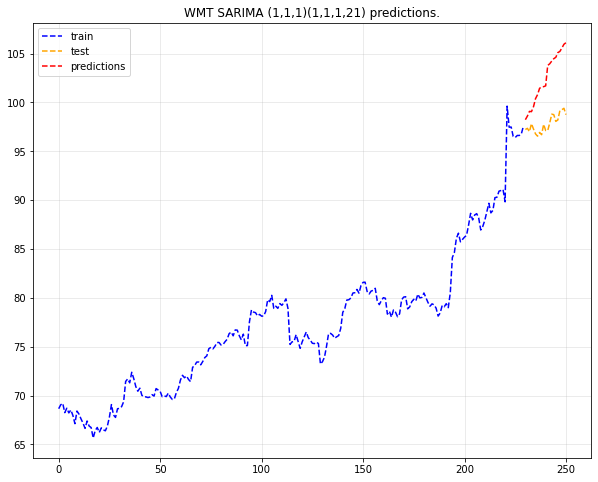
\includegraphics[scale=0.5]{sarima_p3.png}}
\caption{WMT SARIMA (1,1,1)(1,1,1,21) model, training on 2017-1 to 2017-12, predicting 2018-1.}
\end{figure}

\newpage

\section{Final model choices and analysis}\label{section-pred}
Here we compute and compare the mean square error of all model predictions:

\begin{table}[h!]
\begin{tabular}{llll}
\hline
\hline
Mean Square Error            & AAPL  & BA     & WMT   \\
\hline
Double Exponential Smoothing & 102.0 & 4880.2 & 30.1  \\
Triple Exponential Smoothing & 129.3 & 5452.9 & 34.5  \\
ARIMA                        & 101.9 & 4552.2 & 34.4  \\
SARIMA                       & 174.0 & 4242.4 & 532.4  \\
\hline
\hline
\end{tabular}
\end{table}

From the table, we can see that \textbf{ARIMA model works best in general}. Double Exponential Smoothing is also prefered. Two models containing seasonal components (Triple Exponential Smoothing and SARIMA) are less prefered.

\section{Key Findings and Insights}\label{section-find}
The results of the modeling indicates:
\begin{itemize}
\item The stock price series are dominated by upward trend components.
\item The seasonal components is not correctly captured, either it is not important, or it has other external factors contributing.
\item Stock price are not really predictable, the predictions generally have high MSE.
\end{itemize}

\section{Summary and suggestions for next steps}\label{section-sugg}
In summary, this report explores time series modeling on stock prices. The model do capture the general trend, but not the detailed structures of the stock price series.
The problem with the modeling is two fold:
\begin{itemize}
\item They cannot capture seasonality in stock prices correctly, since it is not a simple periodic time stamp.
\item They fail to capture the complex structures.
\end{itemize}
Therefore, the \textbf{possible next steps} include:
\begin{itemize}
\item Use deep learning methods to try to capture the complex seasonality and substructures.
\item Consider what external factors affect stock prices, and involve them into the model.
\end{itemize}

%\bibliographystyle{alpha}
%\bibliography{references} % see references.bib for bibliography management

\end{document}
